\documentclass[11pt]{article}
\usepackage[margin=1in]{geometry}
\usepackage[T1]{fontenc}
\usepackage[utf8]{inputenc}
\usepackage{lmodern}
\usepackage{microtype}
\DisableLigatures{encoding = *, family = *}
\usepackage{booktabs}
\usepackage{graphicx}
\usepackage{url}
\usepackage[hidelinks]{hyperref}
\usepackage{array}
\usepackage{longtable}
\usepackage{amsmath}
\usepackage{caption}
\usepackage{enumitem}
\usepackage{float}
\usepackage{tabularx}
\setlist{nosep}
\sloppy

\title{Internal Role Stability in Voynichese\\\large Morphological Foundations and Multi-Transcription Controls}
\author{Ahaan Kallat\\
Khoury College of Computer Sciences\\
Northeastern University\\
Boston, MA, USA\\
\texttt{kallat.a@northeastern.edu}}
\date{August 31, 2026}

\begin{document}
\maketitle

\begin{abstract}
The Voynich Manuscript is an illustrated medieval codex held by Yale University. Its script has no accepted reading, and the written language is usually called Voynichese. This paper studies a level of structure below grammar and meaning. It asks whether some written units have stable internal roles across the manuscript. A role, in this setting, is a recurring pattern of use inside the text. It is measured from form, position, neighboring context, and manuscript environment.

The study uses a multi-transcription supported core of 1,709 lines and 7,107 token occurrences. Candidate units are built from exact tokens, morphology-aware groups, Stolfi-inspired word-shape signatures, edge signatures, and boundary-merge variants. The analysis then tests those units under controls for manuscript section, textual variety, handwriting group, line position, and tokenization choice. It also uses random baselines, held-out validation, transcription-tier checks, independent clustering, and held-out role prediction.

The promoted catalog covers 1,903 token occurrences, or 26.8 percent of the analyzed core, and appears in 812 lines, or 47.5 percent of analyzed lines. A broader descriptive tier covers 2,175 token occurrences and 858 lines. The result is a reproducible catalog of internal role stability in Voynichese. It gives later grammar and interpretation work a controlled starting point without requiring a proposed decipherment.
\end{abstract}

\noindent\textbf{Keywords} Voynich Manuscript, Voynichese, undeciphered scripts, computational linguistics, morphology, role structure, transcription robustness, confound control, digital humanities.

\section{Introduction}

The Voynich Manuscript is an illustrated medieval codex preserved as Beinecke MS 408 at Yale University Library \cite{yale_ms408}. It contains plant drawings, astronomical and zodiac material, bathing or bodily scenes, pharmaceutical-looking objects, circular diagrams, and a writing system whose contents remain unread. Researchers usually call this writing system Voynichese.

This paper studies Voynichese at an intermediate structural level. The question is whether written units recur in stable roles within the text. A role is a pattern of use. A unit may have a stable role if it appears repeatedly in similar positions, with similar neighbors, or in similar local contexts. The role labels used here are neutral codes such as R06 and R10. They are names for internal patterns, not linguistic labels.

This question is difficult because the manuscript has several known sources of variation. Currier described two major textual varieties, now often called Currier A and Currier B \cite{currier_1976}. Other studies emphasize section differences, scribal hands, page layout, line position, word shape, entropy patterns, and transcription uncertainty \cite{bowern_lindemann_2021}. A recurring form can look important simply because it appears in one section, one textual variety, one handwriting group, or one line position. The analysis treats these factors as controls.

The main output is a catalog of role units with different evidence levels. The promoted catalog covers 26.8 percent of token occurrences and appears in 47.5 percent of analyzed lines. This gives a concrete role layer for future work while keeping the present claim focused on measurable stability.

\section{Contribution and scope}

The paper makes three contributions.

\begin{enumerate}[label=\arabic*.]
\item It defines candidate role units for Voynichese using surface forms, morphology-aware groups, word-shape signatures, edge signatures, and boundary variants.
\item It tests these units under controls for section, textual variety, handwriting group, line position, transcription support, and tokenization choice.
\item It releases a reproducible catalog with promoted role units, exploratory candidates, validation summaries, and scripts.
\end{enumerate}

The study stops at role stability. The next layer is formal grammar, which would test how roles combine into ordered patterns. Interpretation is a later layer that would require evidence from images, diagrams, layout, repeated contexts, or historical comparison.

\section{Layer boundary}

Table~\ref{tablayer} shows the layer covered by this paper. Role stability sits between morphology and formal grammar.

\begin{table}[H]
\centering
\caption{Layer boundary for the present paper}
\label{tablayer}
{\small
\begin{tabular}{ll}
\toprule
Layer & Status in this paper \\
\midrule
Transcription & Used as evidence assumption \\
Morphology & Operational foundation \\
Token families & Role test units \\
Role stability & Main claim \\
Formal grammar & Future work \\
Semantics & Future work \\
\bottomrule
\end{tabular}
}

\end{table}

A stable role can exist before that role has a grammatical or semantic interpretation. For that reason, names such as noun, verb, operator, quantifier, and semantic action are treated as later hypotheses.

\section{Related work}

The analysis builds on several lines of Voynich research. Currier identified large-scale textual differences in Voynichese \cite{currier_1976}. IVTFF and related transcription work make it possible to compare multiple machine-readable versions of the manuscript \cite{zandbergen_transcription}. Stolfi developed detailed models of Voynichese word structure, including prefix, midfix, suffix analysis and later word-grammar work \cite{stolfi_pms_1997,stolfi_word_grammar_2000}. Other computational studies examine entropy, co-occurrence, keywords, and topic structure \cite{reddy_knight_2011,montemurro_zanette_2013,sterneck_topic_2021}. Bowern and Lindemann summarize the linguistic state of the field and the continuing absence of an accepted reading \cite{bowern_lindemann_2021}. Recent work also highlights the need for care when treating glyphs, tokens, and spaces as equivalents of ordinary letters, words, and word spaces \cite{parisel_units_2026}.

This paper uses those results to frame a narrower question. Morphology work informs the candidate units. Currier and section work motivate the controls. Entropy and topic studies show that statistical structure is measurable. The contribution here is to test which written units preserve internal roles across those sources of variation.

\begin{table}[H]
\centering
\caption{Relationship to prior structural work}
\label{tabprior}
\resizebox{\linewidth}{!}{{\scriptsize
\begin{tabular}{lll}
\toprule
Prior layer & Contribution used here & What this paper adds \\
\midrule
Currier & Textual variety is a major confound & Controls role claims against variety \\
IVTFF & Multiple transcription witnesses matter & Uses supported tiers rather than one stream \\
Stolfi & Word internal form is structured & Builds role units from morphology aware lenses \\
Entropy and topics & Large scale structure is measurable & Tests role stability at unit level \\
Recent unit cautions & Tokens and spaces are uncertain & Avoids lexical and grammatical claims \\
\bottomrule
\end{tabular}
}
}
\end{table}

\section{Evidence base}

The input is a line-level Voynich transcription table from the project corpus. It contains 5,376 line records. The primary analysis uses the S1 plus S2 core, which contains 1,709 lines and 7,107 token occurrences across 2,597 surface token types. This core is used because it has support from more than one transcription witness.

The release contains derived project tables and records the external transcription infrastructure as an evidence assumption. Raw third-party transcription witnesses remain external source materials with their own licensing and citation requirements. Table~\ref{tabtranscription} summarizes how transcription evidence is handled.

\begin{table}[H]
\centering
\caption{Transcription assumptions}
\label{tabtranscription}
\resizebox{\linewidth}{!}{{\small
\begin{tabular}{ll}
\toprule
Item & Treatment \\
\midrule
S1 tier & Strict multi transcription core \\
S2 tier & Strong but partial support \\
Raw witnesses & Documented as external sources \\
Unit uncertainty & Handled through morphology lenses and tier checks \\
\bottomrule
\end{tabular}
}
}
\end{table}

Each token occurrence preserves manuscript location, folio, line order, token position, token string, role label, module label, section or illustration code, Currier-like class, hand-like class, line-marker family, and transcription support tier. The main control stratum combines section or illustration code, Currier-like class, hand-like class, and line-marker family.

\section{Morphology foundation}

Surface strings are only one way to define Voynichese units. Prior work shows that Voynichese word forms have strong internal regularities \cite{stolfi_word_grammar_2000}. This study uses that observation to test role stability at several levels of unit definition.

The surface-token definition tests exact transcribed tokens. The conservative morphology definition groups closely related forms. The broad-shape definition groups forms by simplified shape. The Stolfi-inspired definition records gallows pattern, body shape, and terminal class. Additional definitions test edge patterns and possible boundary merges.

\begin{table}[H]
\centering
\caption{Role unit definitions}
\label{tabmorph}
\resizebox{\linewidth}{!}{{\small
\begin{tabular}{ll}
\toprule
Lens & Unit tested \\
\midrule
surface token & Exact token string \\
conservative morphology & Body, terminal class, and reduced body shape \\
broad shape & Reduced body shape and terminal class \\
Stolfi inspired signature & Gallows pattern, reduced remainder shape, and terminal class \\
\bottomrule
\end{tabular}
}
}
\end{table}

These definitions provide a robustness check. A candidate that appears under only one definition is treated cautiously. A candidate that remains supported across several definitions receives stronger evidence.

\section{Internal role layer}

The role labels tested here come from an upstream internal annotation layer. Earlier project work assigned role codes to token occurrences using local context, line position, recurrence, and module structure. This paper evaluates those codes as measurable variables.

For each candidate unit, the analysis measures occurrence count, line support, number of surface types, dominant role, dominant-role share, role entropy, within-stratum role purity, local and global role agreement, spread across control strata, spread across sections, metadata concentration, and module environment.

A unit is promoted when it has enough evidence and passes the relevant reliability checks. Exact surface tokens can be promoted directly. Morphology-based families must contain at least two surface token types, which prevents a family result from restating a single word.

\section{Evaluation design}

The evaluation is designed to rule out simple explanations for apparent role stability. A candidate could look stable because it is frequent, because it has a common word shape, because it appears in one section, because it belongs to one textual variety, because it reflects one handwriting group, because it appears in one line position, because it depends on one transcription tier, or because it depends on one tokenization.

The study uses eight checks.

\begin{enumerate}[label=\arabic*.]
\item Threshold sensitivity reruns the analysis under strict, standard, and loose cutoffs.
\item Ablation tests show how results change when controls are added.
\item Random role baselines break the observed alignment between units and roles.
\item Held-out validation defines units on development data and tests them on held-out lines or folios.
\item Transcription-tier checks compare S1 and S2 evidence.
\item Independent clustering groups units from morphology and context while leaving role labels out of the input features.
\item Held-out role prediction tests whether roles can be recovered from form and local context while manuscript metadata is withheld.
\item Tokenization robustness tests whether promoted units remain supported when unit boundaries are varied.
\end{enumerate}

Together these checks ask whether the analyzed corpus contains a reusable role layer.

\section{Core role stability results}

Table~\ref{tabstatus} gives the standard threshold counts. The surface-token definition yields 16 stable units. The conservative morphology definition yields 1. The broad-shape definition yields 4. The Stolfi-inspired signature definition yields 8. The morphology-based counts are smaller because each supported family must contain more than one surface type and pass the same controls.

\begin{table}[H]
\centering
\caption{Standard role stability counts by unit definition}
\label{tabstatus}
{\small
\begin{tabular}{lrrrr}
\toprule
Lens & Role stable & Local & Contextual & Low power \\
\midrule
broad & 4 & 11 & 62 & 1029 \\
cons morph & 1 & 5 & 61 & 1591 \\
stolfi sig & 8 & 11 & 86 & 1396 \\
surface & 16 & 37 & 64 & 2480 \\
\bottomrule
\end{tabular}
}

\end{table}

\begin{figure}[H]
\centering
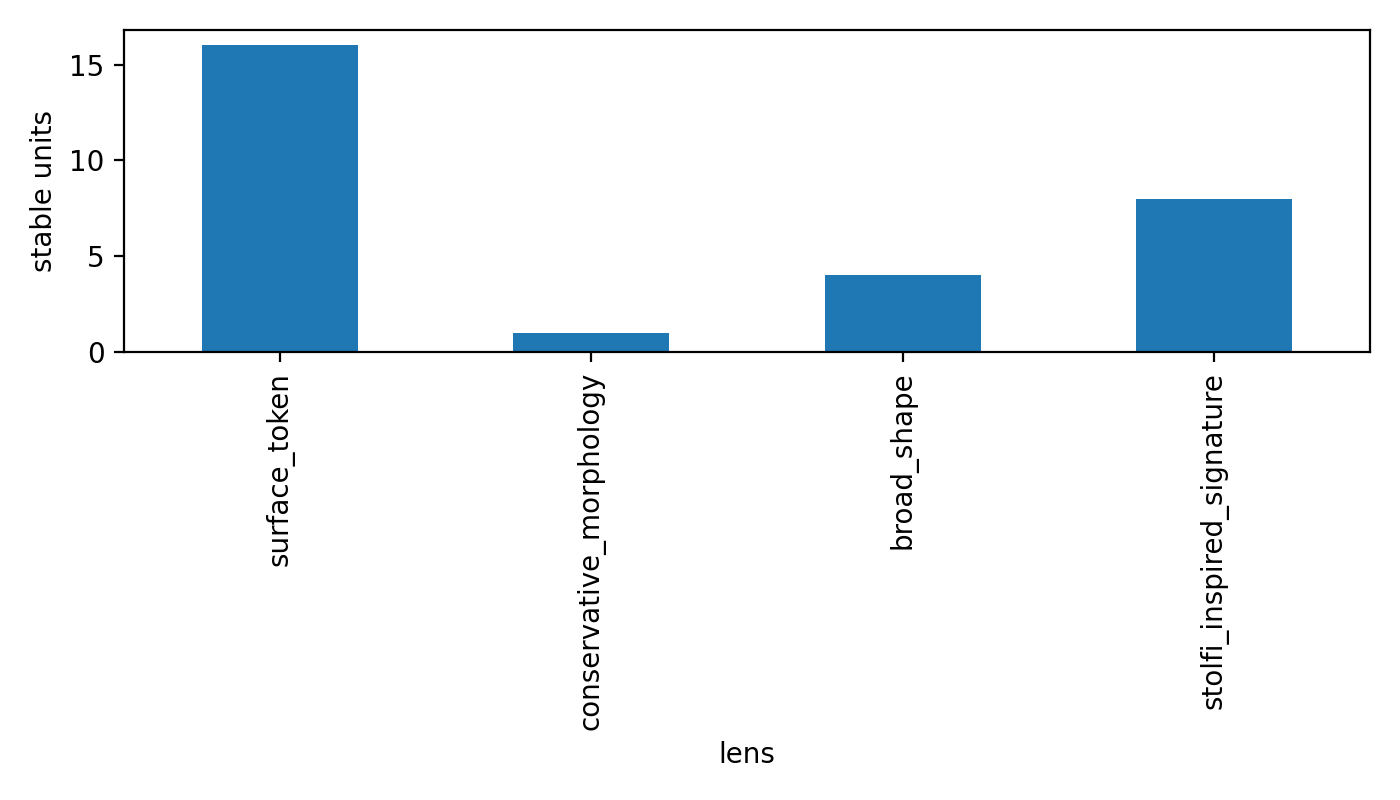
\includegraphics[width=0.78\linewidth]{figures/stable_units_by_lens.png}
\caption{Stable role units by unit definition}
\label{figstable}
\end{figure}

Table~\ref{tabsensitivity} shows how the result changes with cutoff choice. The strict setting keeps a smaller core. The loose setting adds more candidates. The standard setting is used for the main catalog. The same stable core remains visible across settings.

\begin{table}[H]
\centering
\caption{Threshold sensitivity}
\label{tabsensitivity}
{\small
\begin{tabular}{lrrrr}
\toprule
Lens & Strict & Standard & Loose & All three \\
\midrule
broad & 1 & 4 & 13 & 1 \\
cons morph & 0 & 1 & 4 & 0 \\
stolfi sig & 1 & 8 & 15 & 1 \\
surface & 7 & 16 & 32 & 7 \\
\bottomrule
\end{tabular}
}

\end{table}

\begin{figure}[H]
\centering
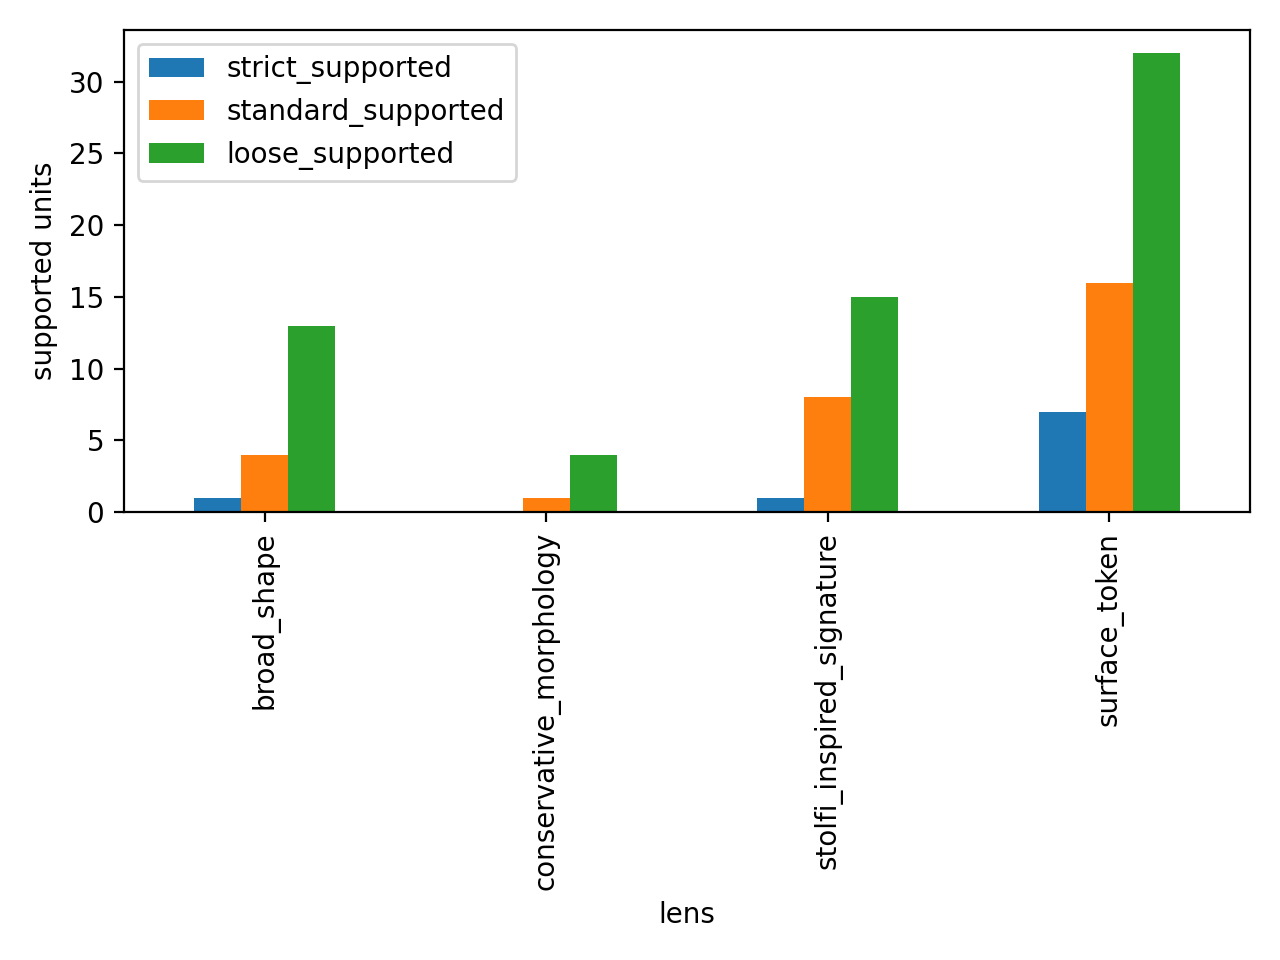
\includegraphics[width=0.82\linewidth]{figures/threshold_sensitivity.png}
\caption{Strict, standard, and loose threshold comparison}
\label{figthreshold}
\end{figure}

Table~\ref{tabablation} shows how many candidates remain as controls are added. Many units satisfy a role-only criterion. Fewer remain after line-marker and full combined controls. The final catalog is therefore more selective than a frequency list or a role-purity list.

\begin{table}[H]
\centering
\caption{Ablation counts under the standard threshold}
\label{tabablation}
{\small
\begin{tabular}{lrrrr}
\toprule
Lens & Role only & Currier & Line marker & Full \\
\midrule
broad & 7 & 6 & 4 & 4 \\
cons morph & 2 & 2 & 1 & 1 \\
stolfi sig & 10 & 9 & 8 & 8 \\
surface & 45 & 37 & 18 & 16 \\
\bottomrule
\end{tabular}
}

\end{table}

\begin{figure}[H]
\centering
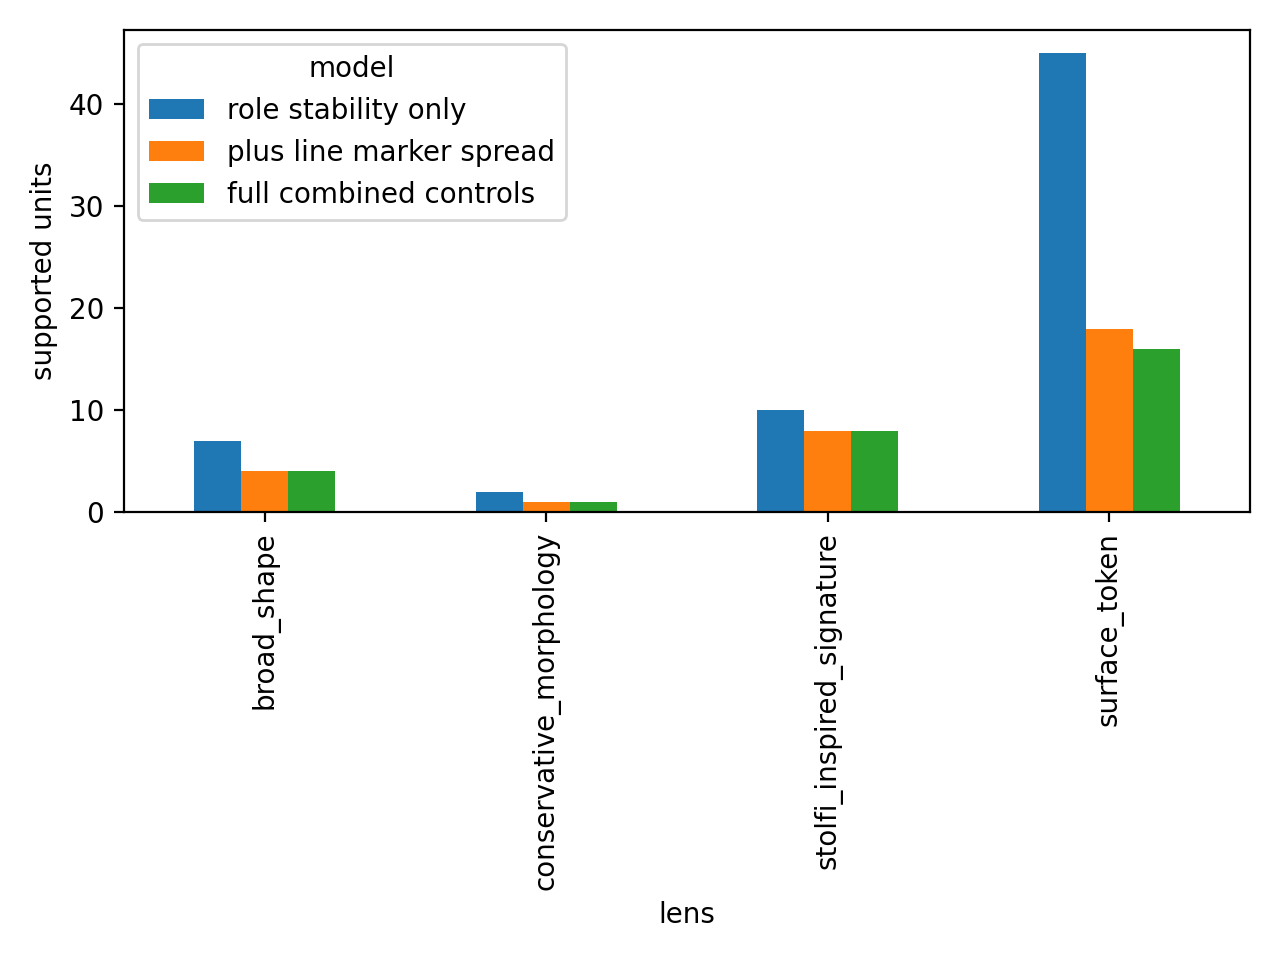
\includegraphics[width=0.86\linewidth]{figures/ablation_counts.png}
\caption{Effect of selected controls on supported units}
\label{figablation}
\end{figure}

\section{Baseline and held-out validation}

Table~\ref{tabbaseline} reports random role baselines. The global role-shuffle baseline recovers no stable units. The within-stratum shuffle baseline recovers almost none. The observed stable units therefore depend on the alignment between written units and role labels.

\begin{table}[H]
\centering
\caption{Random role shuffle baselines}
\label{tabbaseline}
{\small
\begin{tabular}{lrr}
\toprule
Lens & Global shuffle max & Within stratum max \\
\midrule
broad & 0 & 1 \\
cons morph & 0 & 0 \\
stolfi sig & 0 & 0 \\
surface & 0 & 0 \\
\bottomrule
\end{tabular}
}

\end{table}

Table~\ref{tabheldout} reports held-out validation. Units supported on development data are usually observed in held-out data when they have enough coverage. Every development-supported unit that appears in held-out data preserves the same dominant role.

\begin{table}[H]
\centering
\caption{Held-out validation}
\label{tabheldout}
{\small
\begin{tabular}{llrrrr}
\toprule
Basis & Lens & Dev & Seen & Same role & Retained \\
\midrule
folio & broad & 1 & 1 & 1 & 1 \\
folio & stolfi sig & 6 & 6 & 6 & 3 \\
folio & surface & 10 & 10 & 10 & 0 \\
line & broad & 3 & 3 & 3 & 0 \\
line & cons morph & 1 & 1 & 1 & 0 \\
line & stolfi sig & 5 & 5 & 5 & 2 \\
line & surface & 10 & 10 & 10 & 1 \\
\bottomrule
\end{tabular}
}

\end{table}

Table~\ref{tabtier} reports transcription-tier robustness. Every fully supported unit is seen in both S1 and S2 evidence tiers and keeps the same dominant role when observed. S2 is smaller, so fewer units meet frequency thresholds there.

\begin{table}[H]
\centering
\caption{Transcription-tier robustness}
\label{tabtier}
{\small
\begin{tabular}{llrrrr}
\toprule
Tier & Lens & Full & Seen & Same role & Loose \\
\midrule
S1 & broad\_shape & 4 & 4 & 4 & 4 \\
S1 & conservative\_morphology & 1 & 1 & 1 & 1 \\
S1 & stolfi\_inspired\_signature & 8 & 8 & 8 & 5 \\
S1 & surface\_token & 16 & 16 & 16 & 14 \\
S2 & broad\_shape & 4 & 4 & 4 & 0 \\
S2 & conservative\_morphology & 1 & 1 & 1 & 0 \\
S2 & stolfi\_inspired\_signature & 8 & 8 & 8 & 4 \\
S2 & surface\_token & 16 & 16 & 16 & 2 \\
\bottomrule
\end{tabular}
}

\end{table}

\section{Independent role recovery}

Independent recovery addresses the strongest concern about the role labels. The first check clusters candidate units from morphology and context features while leaving role labels out of the clustering input. The role labels are added back only after clustering to measure agreement. Table~\ref{tabinduction} shows agreement across cluster resolutions.

\begin{table}[H]
\centering
\caption{Independent induction agreement}
\label{tabinduction}
{\small
\begin{tabular}{lrrrr}
\toprule
Lens & Standard units & Majority agreement & All resolutions & Mean purity \\
\midrule
broad\_shape & 4 & 3 & 1 & 0.616 \\
conservative\_morphology & 1 & 1 & 0 & 0.531 \\
stolfi\_inspired\_signature & 8 & 6 & 3 & 0.56 \\
surface\_token & 16 & 12 & 7 & 0.702 \\
\bottomrule
\end{tabular}
}

\end{table}

\begin{figure}[H]
\centering
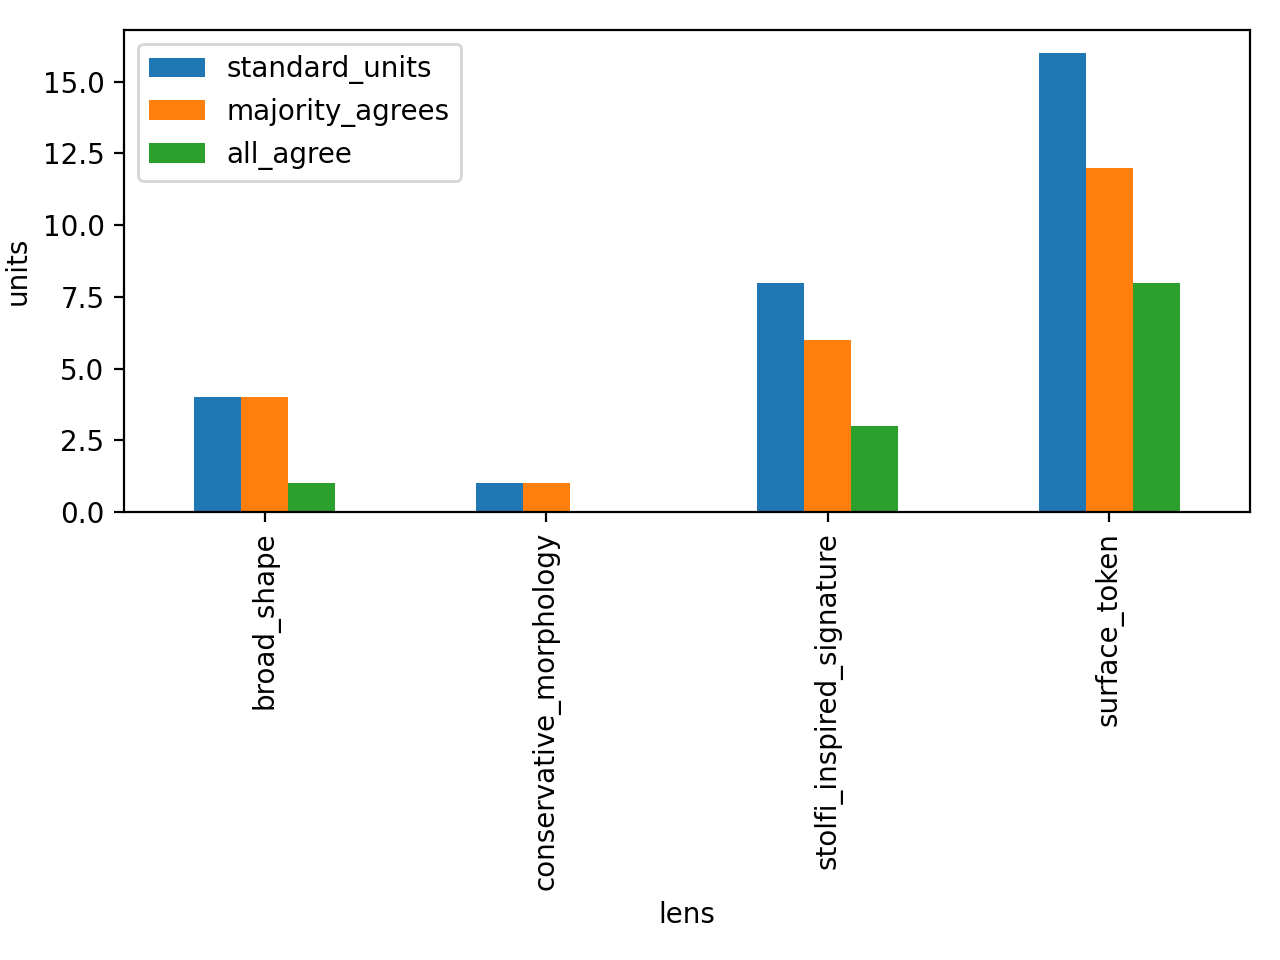
\includegraphics[width=0.86\linewidth]{figures/induction_agreement.png}
\caption{Agreement between induced clusters and audited roles}
\label{figinduction}
\end{figure}

The second check predicts held-out role labels from morphology and context features. Section, textual variety, handwriting group, and line-marker family are not used as input features. Table~\ref{tabpredict} shows that morphology and context outperform majority and position-only baselines. This result suggests that written form and local context carry role information beyond manuscript metadata alone.

\begin{table}[H]
\centering
\caption{Held-out role prediction}
\label{tabpredict}
{\small
\begin{tabular}{llrrrr}
\toprule
Basis & Model & Acc & Bal acc & Macro F1 & Weighted F1 \\
\midrule
folio & majority role baseline & 0.396 & 0.038 & 0.022 & 0.224 \\
folio & position only & 0.142 & 0.068 & 0.033 & 0.2 \\
folio & morphology only & 0.875 & 0.818 & 0.761 & 0.878 \\
folio & morphology plus context & 0.88 & 0.788 & 0.745 & 0.88 \\
line & majority role baseline & 0.387 & 0.042 & 0.023 & 0.216 \\
line & position only & 0.137 & 0.052 & 0.034 & 0.197 \\
line & morphology only & 0.897 & 0.915 & 0.856 & 0.901 \\
line & morphology plus context & 0.886 & 0.8 & 0.738 & 0.887 \\
\bottomrule
\end{tabular}
}

\end{table}

\begin{figure}[H]
\centering
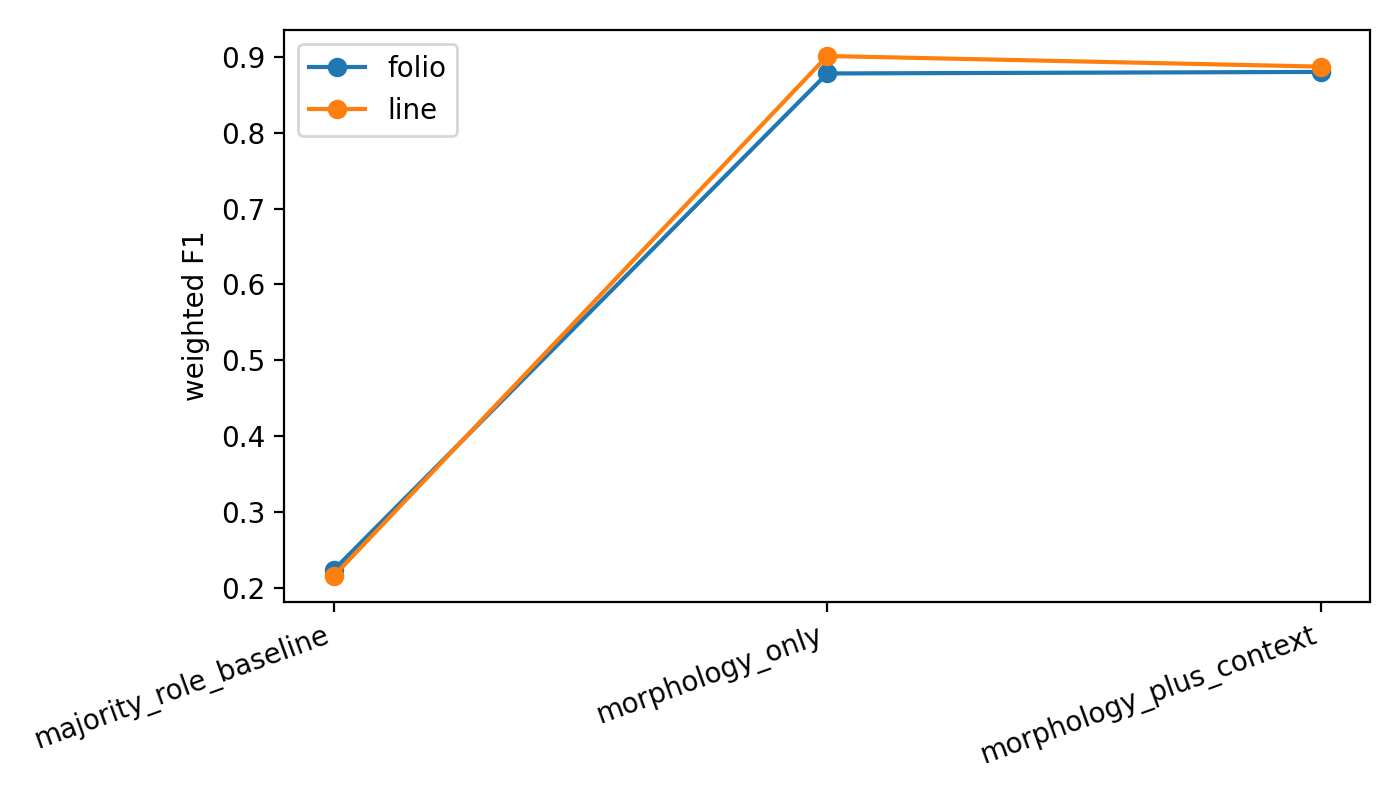
\includegraphics[width=0.86\linewidth]{figures/predictive_validation.png}
\caption{Held-out role prediction by feature set}
\label{figpredict}
\end{figure}

\section{Reliable role catalog}

The reliable catalog has four promoted tiers. A global unit is supported across the full controlled setting. A conditioned unit is supported inside a stated manuscript environment. An environment-sensitive unit has strong local role purity and independent support while being concentrated in one environment. A tokenization-robust unit remains supported under alternate unit-boundary assumptions.

The global catalog contains 23 units. It covers 769 unique token occurrences, which is 10.8 percent of the S1 plus S2 core. It appears in 509 lines, which is 29.8 percent of the core.

\scriptsize
\setlength{\tabcolsep}{3pt}
\begin{longtable}{p{0.19\linewidth}p{0.24\linewidth}p{0.07\linewidth}rrrrp{0.23\linewidth}}
\toprule
Lens & Unit & Role & Occ & Lines & Types & Ind & Top tokens \\
\midrule
\endfirsthead
\toprule
Lens & Unit & Role & Occ & Lines & Types & Ind & Top tokens \\
\midrule
\endhead
broad\_shape & X|NONE & R06 & 46 & 46 & 5 & 2/4 & s, x, g, c, shs \\
broad\_shape & O|dy & R00 & 43 & 43 & 8 & 3/4 & chody, shody, otody, okody, qokody, qotody \\
broad\_shape & OG|y & R00 & 26 & 24 & 8 & 4/4 & choky, choty, otoky, chopy, shoky, oloky \\
conservative\_morphology & o|dy|O & R00 & 41 & 41 & 6 & 3/4 & chody, shody, otody, okody, qokody, qotody \\
stolfi\_inspired\_signature & NG|S\_EY|T\_y & R06 & 104 & 96 & 4 & 4/4 & chey, shey, ey, qey \\
stolfi\_inspired\_signature & NG|S\_OEL|T\_in & R06 & 93 & 82 & 9 & 4/4 & dain, sain, ain, shain, olain, oain \\
stolfi\_inspired\_signature & NG|S\_EY|T\_ey & R06 & 63 & 58 & 6 & 4/4 & sheey, cheey, qoeey, deey, oeey, oleey \\
stolfi\_inspired\_signature & NG|S\_X|T\_NONE & R06 & 46 & 46 & 5 & 2/4 & s, x, g, c, shs \\
stolfi\_inspired\_signature & NG|S\_BY|T\_y & R00 & 33 & 32 & 9 & 3/4 & chy, olchy, dshy, dchy, ochy, orshy \\
stolfi\_inspired\_signature & NG|S\_XY|T\_y & R06 & 30 & 29 & 4 & 3/4 & shy, sy, osy, olsy \\
surface\_token & ar & R06 & 58 & 52 & 1 & 4/4 & ar \\
surface\_token & dar & R06 & 49 & 47 & 1 & 3/4 & dar \\
surface\_token & dain & R06 & 48 & 45 & 1 & 4/4 & dain \\
surface\_token & or & R06 & 48 & 46 & 1 & 4/4 & or \\
surface\_token & shey & R06 & 48 & 46 & 1 & 4/4 & shey \\
surface\_token & okaiin & R10 & 42 & 41 & 1 & 2/4 & okaiin \\
surface\_token & s & R06 & 39 & 39 & 1 & 4/4 & s \\
surface\_token & dal & R09 & 37 & 36 & 1 & 2/4 & dal \\
surface\_token & okain & R10 & 36 & 34 & 1 & 2/4 & okain \\
surface\_token & okal & R07 & 36 & 34 & 1 & 3/4 & okal \\
surface\_token & sheey & R06 & 29 & 28 & 1 & 4/4 & sheey \\
surface\_token & y & R06 & 25 & 25 & 1 & 4/4 & y \\
surface\_token & daiin & R10 & 78 & 67 & 1 & NA & daiin \\
\bottomrule
\end{longtable}


The conditioned catalog adds units that are stable inside a stated environment, mostly textual variety. These units make local structure visible without merging it into the global catalog.

\begin{table}[H]
\centering
\scriptsize
\caption{Conditioned reliable units}
\label{tabconditioned}
\resizebox{\linewidth}{!}{\begin{tabular}{llp{0.18\linewidth}lrrrp{0.23\linewidth}}
\toprule
Scope & Lens & Unit & Role & Occ & New & Lines & Examples \\
\midrule
Currier B & surface & shedy & R06 & 95 & 95 & 83 & shedy \\
Currier B & surface & chedy & R02 & 94 & 94 & 82 & chedy \\
Currier B & surface & qokedy & H12 & 89 & 89 & 73 & qokedy \\
Currier A & surface & daiin & R10 & 81 & 81 & 69 & daiin \\
Currier B & surface & qokeey & H08 & 66 & 66 & 56 & qokeey \\
Currier B & broad\_shape & LB|edy & R00 & 44 & 44 & 42 & lchedy, lshedy, qolchedy, rchedy, qorchedy \\
Currier B & surface & qokaiin & H08 & 37 & 37 & 36 & qokaiin \\
Currier B & surface & okedy & R00 & 33 & 33 & 29 & okedy \\
Currier B & surface & okeedy & R00 & 32 & 32 & 30 & okeedy \\
Currier B & surface & otedy & R01 & 30 & 30 & 28 & otedy \\
Currier B & surface & saiin & R06 & 28 & 28 & 28 & saiin \\
Currier B & surface & qokar & R03 & 26 & 26 & 24 & qokar \\
Currier B & surface & chdy & R02 & 25 & 25 & 24 & chdy \\
\bottomrule
\end{tabular}
}
\end{table}

The environment-sensitive catalog records local evidence when a unit also has strong role purity and independent induction support.

\begin{table}[H]
\centering
\scriptsize
\caption{Environment-sensitive reliable units}
\label{tabenvsensitive}
\resizebox{\linewidth}{!}{\begin{tabular}{lllllllll}
\toprule
Scope & Lens & Unit & Role & Occ & Lines & Votes & New & Top tokens \\
\midrule
localized global & surface token & ol & R06 & 73 & 66 & 5 & 73 & ol \\
localized global & surface token & aiin & R06 & 57 & 51 & 5 & 57 & aiin \\
localized global & surface token & chckhy & R00 & 41 & 39 & 4 & 41 & chckhy \\
localized global & surface token & al & R06 & 31 & 28 & 5 & 31 & al \\
localized global & surface token & oky & R00 & 29 & 29 & 5 & 29 & oky \\
localized global & surface token & sheedy & R06 & 23 & 22 & 5 & 23 & sheedy \\
localized global & broad shape & OXGX|y & R00 & 23 & 23 & 4 & 23 & chocthy, chockhy, shocthy, chocfhy, shockhy \\
localized global & surface token & sho & R06 & 22 & 21 & 5 & 22 & sho \\
localized global & surface token & saiin & R06 & 39 & 38 & 5 & 11 & saiin \\
\bottomrule
\end{tabular}}
\end{table}

\section{Tokenization robustness and coverage}

Visible spaces provide the starting units, and alternate boundaries are tested explicitly. The tokenization check asks whether candidate roles remain supported under surface tokens, morphology units, shape units, edge signatures, and left or right boundary merges.

A tokenization-robust unit is promoted when it has high role purity, independent induction support, and support from at least two unitization variants. This adds coverage while filtering candidates that appear under only one segmentation assumption.

\begin{table}[H]
\centering
\caption{Tokenization robustness summary}
\label{tabtoksummary}
\input{tables/tokenization_robustness_summary.tex}
\end{table}

\begin{figure}[H]
\centering
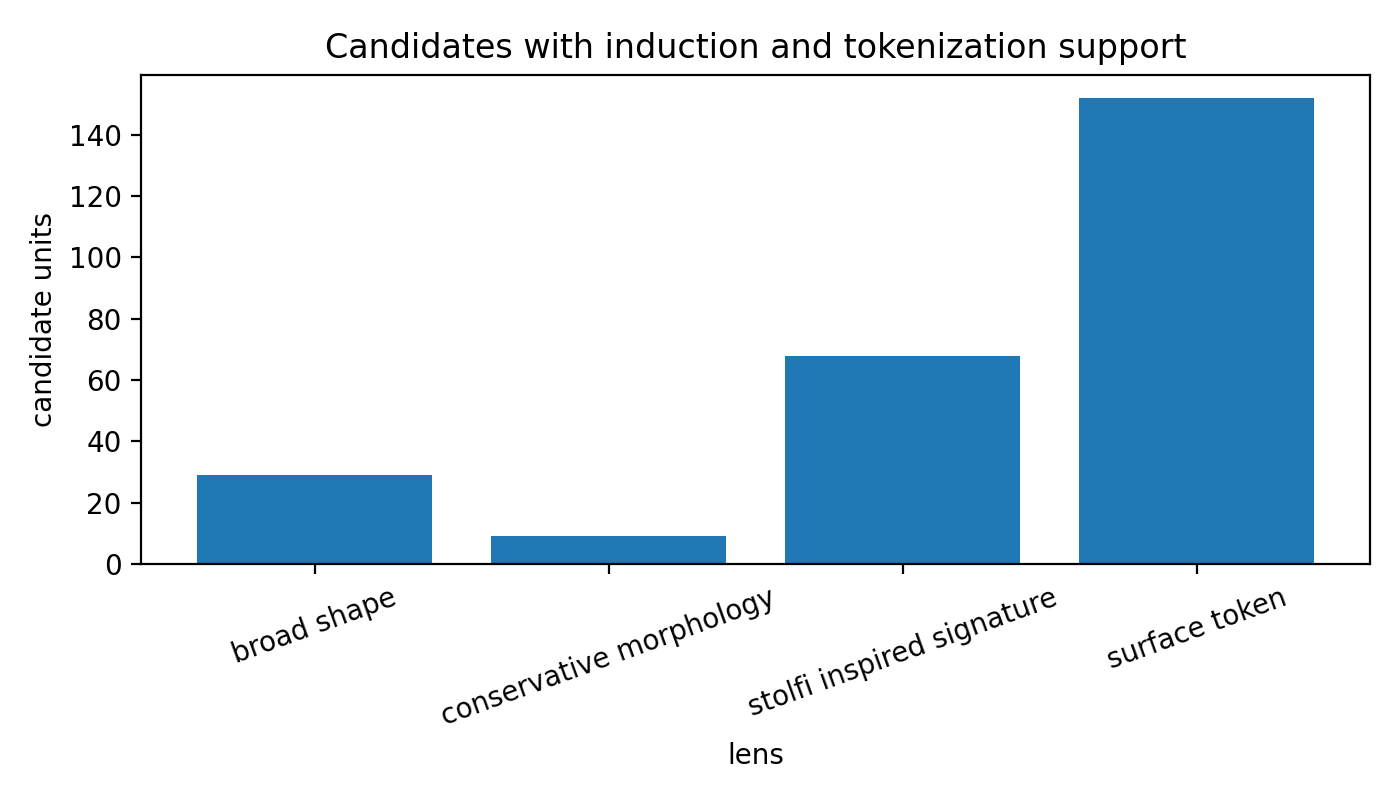
\includegraphics[width=0.82\linewidth]{figures/tokenization_support.png}
\caption{Candidate units with both induction and tokenization support}
\label{figtokensupport}
\end{figure}

\begin{table}[H]
\centering
\scriptsize
\caption{Tokenization-robust reliable units}
\label{tabtokcat}
\resizebox{\linewidth}{!}{\input{tables/tokenization_robust_reliable_catalog.tex}}
\end{table}

The full promoted layer covers 1,903 token occurrences, which is 26.8 percent of the core. It touches 812 lines, which is 47.5 percent of the core. The promising unpromoted tier adds 272 further occurrences for descriptive coverage. With that tier included, the descriptive layer covers 2,175 token occurrences and touches 858 lines.

\begin{table}[H]
\centering
\scriptsize
\caption{Coverage by reliability tier}
\label{tabcoverage}
\resizebox{\linewidth}{!}{\begin{tabular}{lrrrrrrrr}
\toprule
Tier & Tok & Tok \% & Lines & Line \% & Cum tok & Cum tok \% & Cum lines & Cum line \% \\
\midrule
Global reliable & 769 & 10.82 & 509 & 29.78 & 769 & 10.82 & 509 & 29.78 \\
Conditioned reliable & 680 & 9.57 & 382 & 22.35 & 1449 & 20.39 & 693 & 40.55 \\
Environment sensitive & 310 & 4.36 & 257 & 15.04 & 1759 & 24.75 & 759 & 44.41 \\
Tokenization robust & 144 & 2.03 & 133 & 7.78 & 1903 & 26.78 & 812 & 47.51 \\
Promising unpromoted & 272 & 3.83 & 219 & 12.81 & 2175 & 30.60 & 858 & 50.20 \\
Low or unassigned & 4932 & 69.40 & 1584 & 92.69 & 7107 & 100.00 & 1709 & 100.00 \\
\bottomrule
\end{tabular}}
\end{table}

\begin{figure}[H]
\centering
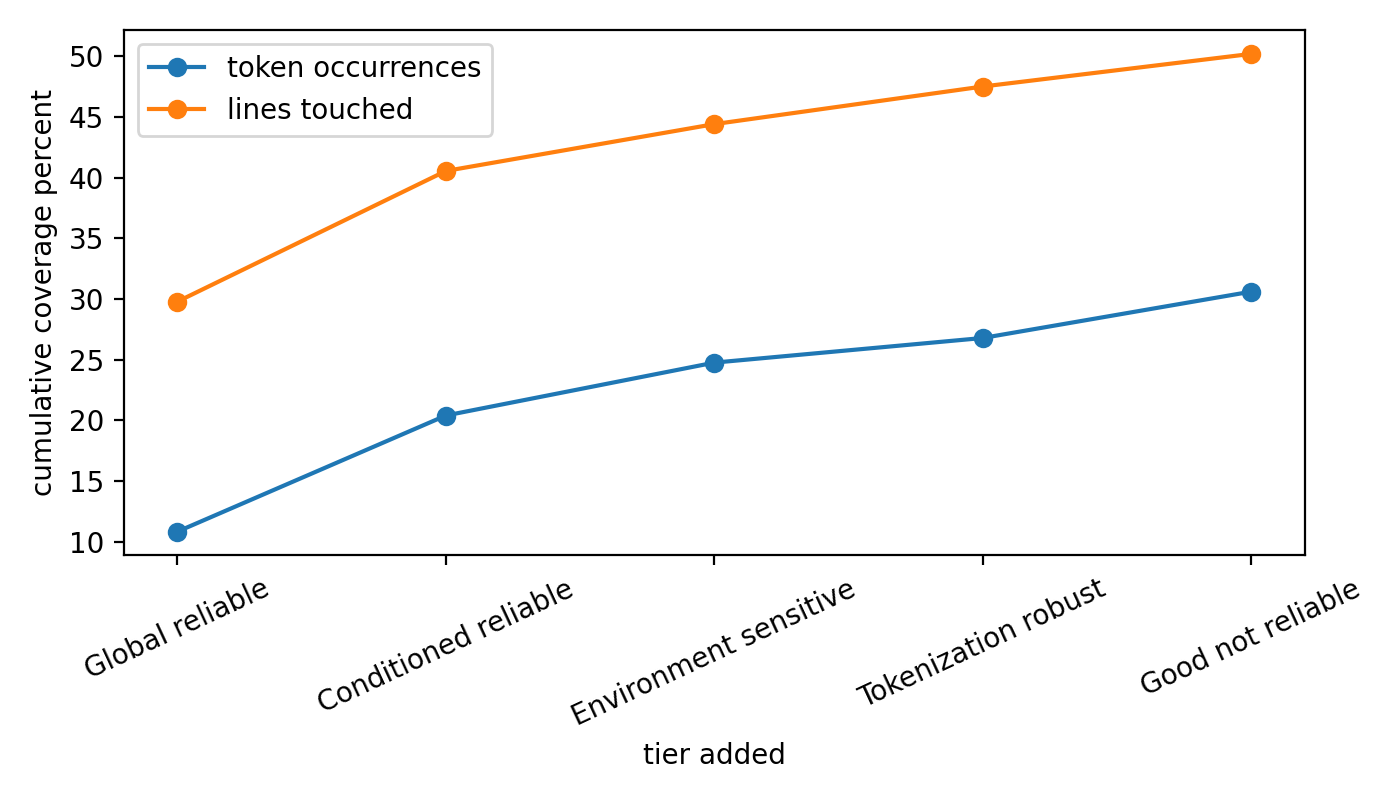
\includegraphics[width=0.80\linewidth]{figures/cumulative_coverage.png}
\caption{Cumulative coverage after adding each reliability tier}
\label{figcoverage}
\end{figure}

The promising tier is retained for transparency. These units often show plausible role behavior while missing at least one promotion check, such as induction support, tokenization support, role purity, or evidence size.

\begin{table}[H]
\centering
\scriptsize
\caption{Largest promising unpromoted units}
\label{tabgood}
\resizebox{\linewidth}{!}{\begin{tabular}{lllrrrrrrl}
\toprule
Scope & Lens & Unit & Role & Occ & Lines & Ind & Tokn & New & Reason \\
\midrule
global & surface token & daiin & R10 & 134 & 116 & 1 & 2 & 53 & low induction \\
line\_marker paragraph\_continuation & surface token & daiin & R10 & 126 & 108 & 1 & 2 & 50 & low induction \\
global & broad shape & EXGX|y & R00 & 25 & 25 & 0 & 2 & 25 & low induction \\
currier B & stolfi inspired signature & NG|S\_OL|T\_r & R06 & 143 & 113 & 5 & 2 & 23 & low purity \\
hand 2 & surface token & daiin & R10 & 23 & 19 & 1 & 2 & 23 & low induction \\
hand 2 & surface token & qokal & H08 & 23 & 21 & 1 & 2 & 23 & low induction \\
line\_marker paragraph\_continuation & broad shape & EXGX|y & R00 & 23 & 23 & 0 & 2 & 23 & low induction \\
currier\_hand B|2 & surface token & daiin & R10 & 23 & 19 & 1 & 2 & 23 & low induction \\
currier\_hand B|2 & surface token & qokal & H08 & 23 & 21 & 1 & 2 & 23 & low induction \\
currier B & broad shape & EXGX|y & R00 & 21 & 21 & 0 & 2 & 21 & low induction \\
currier\_marker B|paragraph\_continuation & broad shape & EXGX|y & R00 & 21 & 21 & 0 & 2 & 21 & low induction \\
currier\_marker B|paragraph\_continuation & stolfi inspired signature & NG|S\_OL|T\_r & R06 & 137 & 107 & 5 & 2 & 20 & low purity \\
\bottomrule
\end{tabular}}
\end{table}

\begin{table}[H]
\centering
\scriptsize
\caption{Role coverage across reliability tiers}
\label{tabrolecoverage}
\resizebox{\linewidth}{!}{\input{tables/role_coverage_summary.tex}}
\end{table}

\section{Section-level roles and role switching}

The manuscript is section-sensitive. Table~\ref{tabsection} and Figure~\ref{figsection} show that role mixtures differ by section code. These differences support the use of section as a control and provide a descriptive basis for future grammar work.

\begin{table}[H]
\centering
\caption{Section-level role profiles}
\label{tabsection}
{\small
\begin{tabular}{lrrrrrr}
\toprule
Section & Occ & Lines & Top role & Share & Second & Share \\
\midrule
H & 1893 & 340 & R06 & 0.353 & R00 & 0.339 \\
S & 1872 & 207 & R00 & 0.407 & R06 & 0.27 \\
B & 1512 & 271 & R00 & 0.335 & R06 & 0.295 \\
T & 467 & 96 & R06 & 0.353 & R00 & 0.336 \\
P & 428 & 216 & R00 & 0.533 & R06 & 0.236 \\
C & 403 & 197 & R00 & 0.514 & R06 & 0.323 \\
A & 295 & 161 & R00 & 0.59 & R06 & 0.315 \\
Z & 237 & 221 & R00 & 0.789 & R06 & 0.127 \\
\bottomrule
\end{tabular}
}

\end{table}

\begin{figure}[H]
\centering
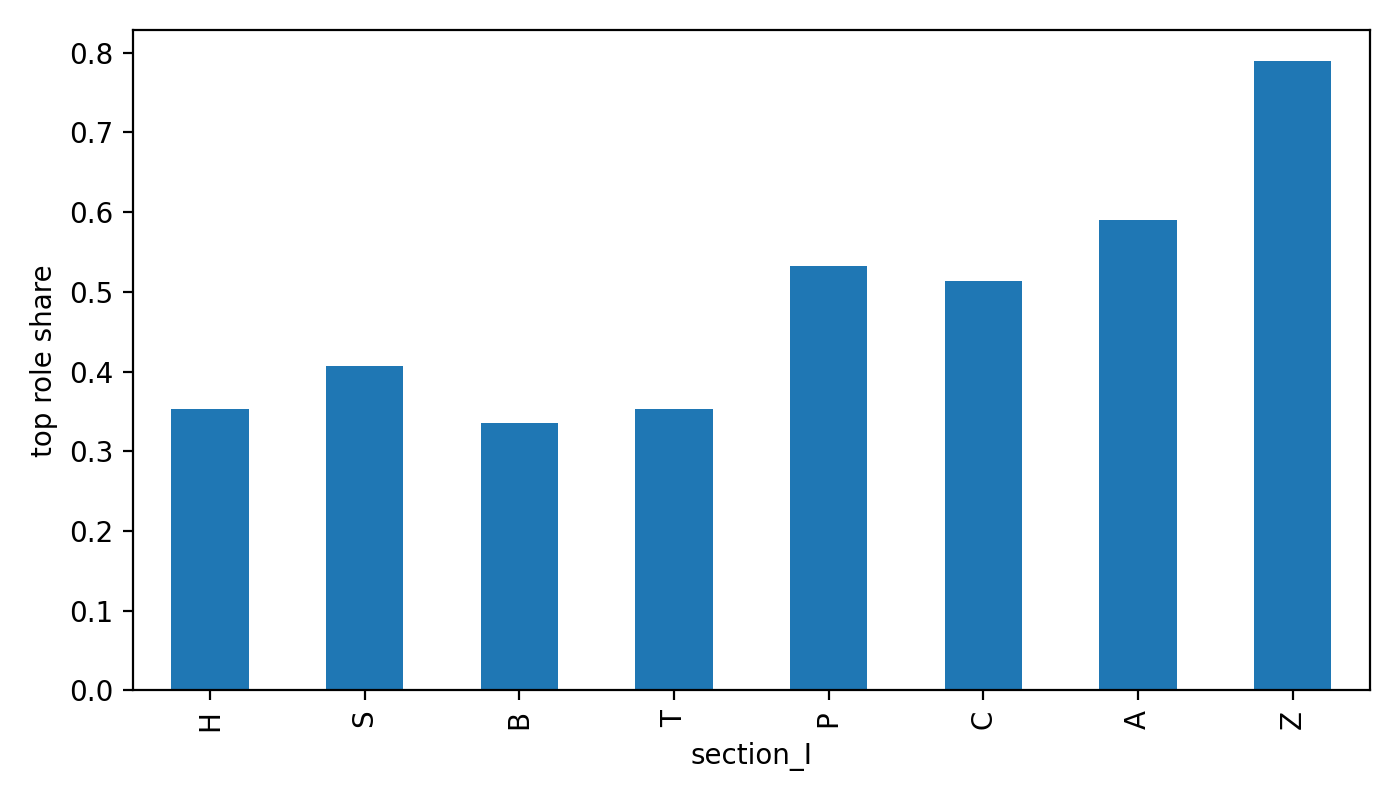
\includegraphics[width=0.84\linewidth]{figures/section_role_profiles.png}
\caption{Top role shares by section code}
\label{figsection}
\end{figure}

The analysis also checks whether the same unit receives different reliable roles in different local scopes. The method allows such cases. Under the current promotion rules, no high-confidence role-switching case is found. Role switching therefore remains a target for larger or more detailed evidence bases.

\begin{table}[H]
\centering
\caption{Role switching audit}
\label{tabroleswitch}
\input{tables/role_switch_audit.tex}
\end{table}

\section{Future hypotheses}

The stable role units can support more specific hypotheses in later work. Some roles may eventually prove useful for studying operator-like, terminal-like, quantifier-like, or procedure-like patterns. Table~\ref{tabhypotheses} records these possibilities as future tests.

\begin{table}[H]
\centering
\caption{Future hypotheses outside the current claim}
\label{tabhypotheses}
\resizebox{\linewidth}{!}{{\small
\begin{tabular}{ll}
\toprule
Hypothesis & Required future test \\
\midrule
Operator like roles & Show ordered transitions and action like distribution \\
Terminal like roles & Show termination beyond line position effects \\
Quantifier like roles & Show count or measure behavior from external anchors \\
Procedure like structure & Show formal sequence rules across held out pages \\
\bottomrule
\end{tabular}
}
}
\end{table}

The present result rests on the stability tests. Future studies can use the catalog to test formal grammar, section-specific syntax, and image-linked interpretation.

\section{Limitations}

The role labels come from an upstream internal annotation layer. Independent clustering and held-out prediction reduce that dependence. A future study could rebuild the full layer from raw manuscript images and individual transcription witnesses.

The morphology layer is operational. It is based on known word-structure ideas and functions here as a testing framework. Complete historical morphology remains a separate task. Conditioned and environment-sensitive units provide local role evidence rather than global role evidence. Transcription-tier robustness uses support tiers rather than a full leave-one-witness-out design, because the available project table records support tiers instead of all individual witness strings. Held-out tests are also affected by frequency, since small held-out sets can remove otherwise consistent units from the measurable range.

These limits define the strength of the claim. The paper establishes a role-stability layer that can be rerun, challenged, and extended. Formal grammar and interpretation require separate follow-up studies.

\section{Conclusion}

This paper presents a morphology-aware and multi-transcription controlled account of internal role stability in Voynichese. The promoted catalog survives combined controls, threshold checks, ablations, random role baselines, held-out validation, transcription-tier checks, section profiling, independent clustering, held-out prediction, and tokenization robustness checks.

The result is a reproducible role layer for later grammar work. Language identification, lexical interpretation, phonetic values, formal grammar, and semantics remain future stages with their own evidence requirements.

\section*{Acknowledgments}

AI tools were used for drafting support, code organization, LaTeX packaging, and exploratory analysis assistance. The author reviewed and finalized the methods, wording, reported results, code release, and interpretation.

\section*{Code and data availability}

The code, derived data, and paper source are available at \url{https://github.com/ahaankallat/voynich-role-stability}.

\clearpage
\begin{thebibliography}{99}

\bibitem{yale_ms408}
Yale University Library. Beinecke MS 408. Voynich Manuscript. Yale University Library Digital Collections.

\bibitem{currier_1976}
Currier, Prescott H. 1976. Papers on the Voynich Manuscript. Edited by Mary E. D'Imperio. National Security Agency.

\bibitem{zandbergen_transcription}
Zandbergen, Rene. The Voynich Manuscript. Transliteration of the text. Voynich.nu.

\bibitem{stolfi_pms_1997}
Stolfi, Jorge. 1997. Prefix midfix suffix decomposition of Voynichese words. Voynich Manuscript notes.

\bibitem{stolfi_word_grammar_2000}
Stolfi, Jorge. 2000. A Grammar for Voynichese Words. Voynich Manuscript notes.

\bibitem{reddy_knight_2011}
Reddy, Sravana and Kevin Knight. 2011. What We Know About The Voynich Manuscript. Proceedings of the ACL Workshop on Language Technology for Cultural Heritage, Social Sciences, and Humanities.

\bibitem{montemurro_zanette_2013}
Montemurro, Marcelo A. and Damian H. Zanette. 2013. Keywords and Co Occurrence Patterns in the Voynich Manuscript. PLOS ONE 8. e66344.

\bibitem{bowern_lindemann_2021}
Bowern, Claire and Luke Lindemann. 2021. The Linguistics of the Voynich Manuscript. Annual Review of Linguistics 7. 285 to 308.

\bibitem{sterneck_topic_2021}
Sterneck, Rachel, Annie Polish, and Claire Bowern. 2021. Topic Modeling in the Voynich Manuscript. arXiv 2107.02858.

\bibitem{parisel_currier_2026}
Parisel, Christophe. 2026. A Quantitative Confirmation of the Currier Language Distinction. arXiv 2604.25979.

\bibitem{parisel_units_2026}
Parisel, Christophe. 2026. A Glyph Is Not a Letter, a Token Is Not a Word, a Space Is Not a Space. arXiv 2608.17096.

\end{thebibliography}


\end{document}
